%%%%%%%%%%%%%%%%%%%%%%%%%%%%%%%%%%%%%%%%%
% University/School Laboratory Report
% LaTeX Template
% Version 3.1 (25/3/14)
%
% This template has been downloaded from:
% http://www.LaTeXTemplates.com
%
% Original author:
% Linux and Unix Users Group at Virginia Tech Wiki 
% (https://vtluug.org/wiki/Example_LaTeX_chem_lab_report)
%
% License:
% CC BY-NC-SA 3.0 (http://creativecommons.org/licenses/by-nc-sa/3.0/)
%
%%%%%%%%%%%%%%%%%%%%%%%%%%%%%%%%%%%%%%%%%

%----------------------------------------------------------------------------------------
%	PACKAGES AND DOCUMENT CONFIGURATIONS
%----------------------------------------------------------------------------------------

\documentclass{article}

\usepackage{graphicx} % Required for the inclusion of images
\usepackage{natbib} % Required to change bibliography style to APA
\usepackage{amsmath} % Required for some math elements 
\usepackage{listings}
\usepackage{color}
\usepackage[margin=1in]{geometry}

\definecolor{dkgreen}{rgb}{0,0.6,0}
\definecolor{gray}{rgb}{0.5,0.5,0.5}
\definecolor{mauve}{rgb}{0.58,0,0.82}

\lstset{frame=tb,
  language=R,
  aboveskip=3mm,
  belowskip=3mm,
  showstringspaces=false,
  columns=flexible,
  basicstyle={\small\ttfamily},
  numbers=none,
  numberstyle=\tiny\color{gray},
  keywordstyle=\color{blue},
  commentstyle=\color{dkgreen},
  stringstyle=\color{mauve},
  breaklines=true,
  breakatwhitespace=true,
  tabsize=3
}
\setlength\parindent{0pt} % Removes all indentation from paragraphs

\renewcommand{\labelenumi}{\alph{enumi}.} % Make numbering in the enumerate environment by letter rather than number (e.g. section 6)

%----------------------------------------------------------------------------------------
%	DOCUMENT INFORMATION
%----------------------------------------------------------------------------------------

\title{Project 1 \\ STAT 355} % Title
\author{Sabbir \textsc{Ahmed}} % Author name
\date{\today} % Date for the report

\begin{document}

    \maketitle % Insert the title, author and date

    % If you wish to include an abstract, uncomment the lines below
    % \begin{abstract}
    % Abstract text
    % \end{abstract}

    %----------------------------------------------------------------------------------------
    %	SECTION 1
    %----------------------------------------------------------------------------------------

    \section{Objective}
    To determine the atomic weight of magnesium via its reaction with oxygen and to study the stoichiometry of the reaction (as defined in \ref{definitions}):

        \subsection{Definitions}
        \label{definitions}
            \begin{description}
                \item[Stoichiometry]
                The relationship between the relative quantities of substances taking part in a reaction or forming a compound, typically a ratio of whole integers.
                \item[Atomic mass]
                The mass of an atom of a chemical element expressed in atomic mass units. It is approximately equivalent to the number of protons and neutrons in the atom (the mass number) or to the average number allowing for the relative abundances of different isotopes. 
            \end{description} 

    %----------------------------------------------------------------------------------------
    %	SECTION 2
    %----------------------------------------------------------------------------------------

    \section{Part 1}
        1000 random numbers were generated using a Bernoulli random variable with n = 20, p = 0.4
\begin{lstlisting}
    # main.R
    # initializing variables
    x <- 20
    N <- 1000
    p <- 0.4
    generatedData <- rbinom(N, x, p)
\end{lstlisting}

        \subsection{Distribution}
            Distribution of the data was plotted with a histogram using ggplot2
\begin{lstlisting}
    # plot a histogram
    ggplot() + aes(generatedData) + geom_histogram(binwidth=1, colour="black", fill="white")
\end{lstlisting}

            \begin{figure}[h]
                \begin{center}
                    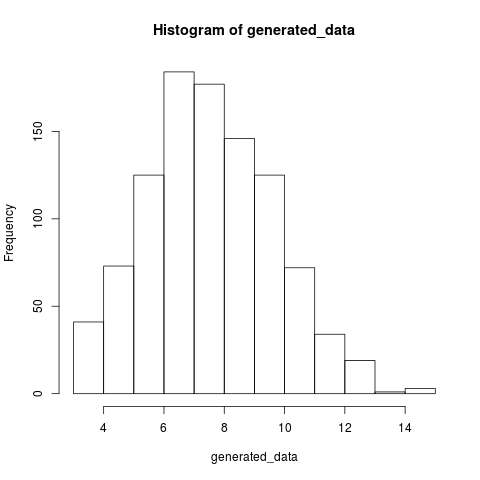
\includegraphics[width=0.6\textwidth]{hist} % Include the image placeholder.png
                    \caption{Histogram of the Generated Data}
                \end{center}
            \end{figure}

        \subsection{Mean, Variance, and Standard Deviation}
            The mean, variance and standard deviation of the data were computed with the following snippet
\begin{lstlisting}
    # print out the mean, variance and standard deviation
    paste("Mean:", signif(mean(generatedData), digits=4),
        "| Variance:", signif(var(generatedData), digits=4),
        "| Standard Deviation:", signif(sqrt(var(generatedData)), digits=4))
\end{lstlisting}

        \subsection{Summary}
            Summary statistics were generated with the following snippet
\begin{lstlisting}
    # print out the summary statistics
    summary(generatedData)
\end{lstlisting}

\end{document}